\documentclass{sig-alternate}

% UTF8 support
\usepackage[utf8x]{inputenc}

\usepackage{tikz}
\usetikzlibrary{positioning}


\usepackage{hyperref}
\usepackage{epsf,graphicx}
\graphicspath{{figures/}}
\usepackage{subfig}
\usepackage[colorinlistoftodos]{todonotes}

\newcommand{\eg}{{\textit{e.g.~}}}
\newcommand{\etal}{{\textit{et al.~}}}
\newcommand{\ie}{{\textit{i.e.~}}}

%
% --- Author Metadata here ---
\conferenceinfo{10th ACM/IEEE International Conference on Human-Robot Interaction}{2015 Portland, USA}
%\CopyrightYear{2007} % Allows default copyright year (20XX) to be over-ridden - IF NEED BE.
%\crdata{0-12345-67-8/90/01}  % Allows default copyright data (0-89791-88-6/97/05) to be over-ridden - IF NEED BE.
% --- End of Author Metadata ---


\title{\LARGE \bf
    Designed to survive a nursery
}


%%% HRI 2015 -> double-blind review process

%\numberofauthors{3} 
%\author{
%\alignauthor
%Séverin Lemaignan\\
%Julia Fink\\
%Pierre Dillenbourg\\
%    \affaddr{Computer-Human Interaction in\\ Learning and Instruction (CHILI)}\\
%    \affaddr{Ecole Polytechnique Fédérale\\ de Lausanne (EPFL)}\\
%    \affaddr{CH-1015 Lausanne, Switzerland}\\
%    \email{firstname.lastname@epfl.ch}
%\alignauthor
%Francesco Mondada\\
%    \affaddr{Computer-Human Interaction in\\ Learning and Instruction (CHILI)}\\
%    \affaddr{Ecole Polytechnique Fédérale\\ de Lausanne (EPFL)}\\
%    \affaddr{CH-1015 Lausanne, Switzerland}\\
%    \email{firstname.lastname@epfl.ch}
%\alignauthor
%Florian Wille\\
%Karmen Franinovi\'c\\
%   \affaddr{Z\"urcher Hochschule der K\"unste (ZHdK)}\\
%   \affaddr{Z\"urich, Switzerland}
%}
%


\begin{document}



\maketitle

\begin{abstract}

This paper presents the concept and an example of \textit{robject}, a robotic
entity embedded in an everyday object.  Robjects use the affordance of the
original object to ensure an efficient interaction and a high acceptance.  The
example of the \textit{ranger robot} shows that this approach can be applied to
the domestic environment.  We explore the integration of a robot
(\textit{robject}) into a family household, by regarding the home as a
ecosystem, which consists of people, parts, products, activities, and
interactions.  A test of the \textit{ranger robot} in families validates this
holistic approach and shows the impact of this type of design in respect to the
complexity of the robotic system.

\keywords{holistic approach, ecosystem, cooperation with humans, domestic service robots, robject, ranger robot}
\end{abstract}
%
\section{Introduction}
%
Since years, predictions say service robotics will massively enter in every home
\cite{Gates2007}.  In Europe, a large survey made in 2012 shows a general public
perception which is still not very open to home service robotics.  Robots are
perceived as a good tool mainly for dangerous tasks \cite{Eurobarometer2012}.
In the same survey, a majority of people thinks robots should be banned from
typical home service scenarios that include children, elderly or disabled care.
Only 13\% of the European citizen think robots should be applied in priority to
``domestic use, such as cleaning''.  Also among researchers it has not been
clear what a robot exactly should do in homes \cite{Pantofaru2012}.  Pantofaru
et al. \cite{Pantofaru2012} explored the role of robots in home organization
(tidying, storing), and found that robots could have a potentially high impact
on this.  Similarly, Bell et al. \cite{Bell2005} suggest that robots could be
used in tidying up scenarios in the domestic environment.

Although only few such systems have entered the consumer market, several
researchers took advantage of these few success and studied the acceptance of
robotics technology by the users.  Bauwens et al. \cite{Bauwens2012} showed that
the main factors impacting the adoption of robotics at home are, from the most
to the less important:

\begin{enumerate}
\item The practical utility
\item The integration into the home ecosystem (physical space, users, habits)
\item The economic utility
\end{enumerate}

Most of the service robots developed in research only look at a subset of these
criteria, approaching single disciplines such as HRI, mechatronics or robotic
functionality.

In this paper we present an holistic approach and an example of mechatronic
implementation looking for a balance between functionality, cost and integration
into the ecosystem.  We believe that an holistic and interdisciplinary approach
can improve acceptance and bring robotics in homes in a faster and more
efficient way.  Our approach consists in integrating robotics technology into
daily objects, making them what we call \textit{robjects}.  Robjects can easily
blend into the home ecosystem because of the embodiment in an object that is
already integrated into the ecosystem and has a clear function in it.  Robjects
also aim at a close synergy with the users, replacing high technological
requirements with better human-robot interaction for collaboration.  These
principles have already been applied to some successful systems in industry, as
illustrated in section \ref{sec:sota}. Section \ref{sec:ranger} presents an
example of robject and the first results of user tests.


\section{State of the art}
\label{sec:sota}

In homes, research aims at adding intelligence into home automation, for
instance to implement user activity recognition \cite{duque2013knowledge} and
integrate service robots \cite{Cavallo2013}.  In most cases this technology,
which is still very heavy, targets assistive living for elderly.  A set of
European research projects work exactly on this issue:
Robot-ERA\cite{Aquilano2012} is developing several service robots for indoor and
outdoor use, integrated in smart houses and providing a set of services for
older people, Giraffe+\cite{Coradeschi2013} integrates a telepresence robot into
a smart home where the sensor network allows context recognition and
interpretation of collected data, ACCOMPANY\cite{Accompany2013} develops a
robotic companion integrated into an intelligent environment, providing services
to elderly users to enable independent living at home, MOBISERV\cite{Nani2010}
aims at studying innovative technology to support independent living of older
adults at home or in specialized institutions, CompanionAble\cite{Gross2011} has
worked on the synergy between robotics and ambient Intelligence technologies
enabling a care-giver's assistive environment and
HOBBIT\cite{fischinger2013hobbit} develops a socially assistive robot that helps
elderly at home.  All these projects involve robots that have a human-like
presence in the environment.  Few projects such as RUBICON\cite{Bacciu2013} have
a more general approach and study a more generic network of sensors and
actuators, without a predefined aapplication of assisted living in mind.
Finally only very few consider the interaction with children.  The MOnarCH
project \cite{Sequeira2013} is studying the interaction with children in
hospitals with a smaller robot, still having a human-like shape.  Their study on
interaction is probably one of the closest to our project. 

The integration of designers in research projects to study interaction aspects
and gather information on new approaches is very recent in the field.  A good
experiment has been carried out in the University of Hertfordshire Robot House,
where artists lived full-time with various robots in a smart home environment
\cite{LEHMANN2013}.  This approach gives many insights on interactions aspects,
as we saw in our project.

Although most of the service robots developed in research lab do not meet market
requirements or address only part of the requirements, few managed to become
successful products.  Among them we can find the Kiva systems \cite{Wurman2008}
or the Baxter robot \cite{Fitzgerald2013}, both systems focusing on cooperation
with humans, functional shapes, low cost and high added value functionalities.
This situation confirms what Takayama et al. \cite{Takayama2008} found: ``people
would feel more positively toward robots doing occupations \textit{with} people
rather than \textit{in place} of people''.  Transposing this approach to homes
for a use with children, we developed a robot to help tidying-up the children's
room, which has been considered as an interesting task by previous studies
\cite{Pantofaru2012,Bell2005}.

\begin{figure*}[t]
 \centering
    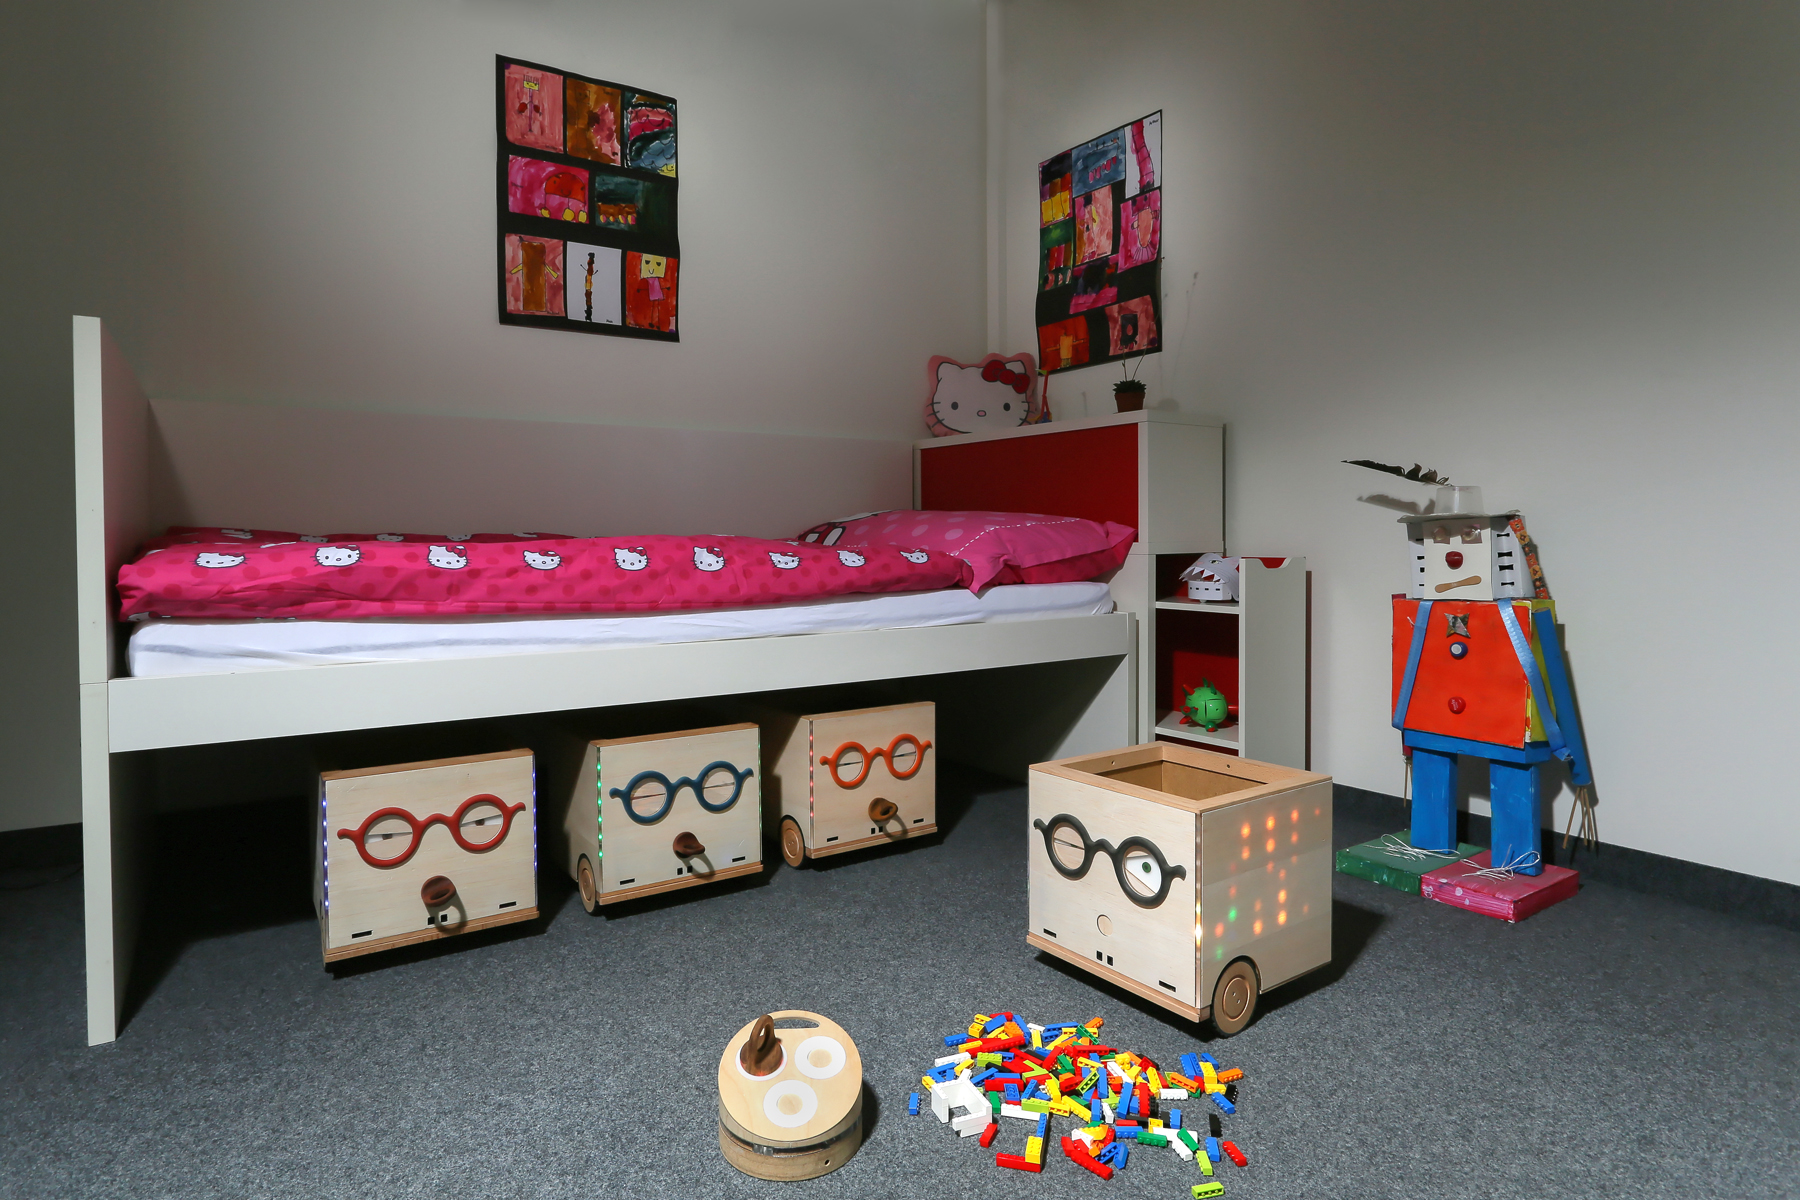
\includegraphics[width=0.9\columnwidth]{ranger-room.jpg}
  \caption{A set of ranger robots in a room. Their home is under the bed, where they sleep recharging their battery. Photo: Alain Herzog.}
  \label{fig:ranger_room} 
\end{figure*}

\begin{figure*}
    \centering
    \begin{tikzpicture}[
        >=latex,
        scale=1]
        \node[anchor=north] at (0,0)
            {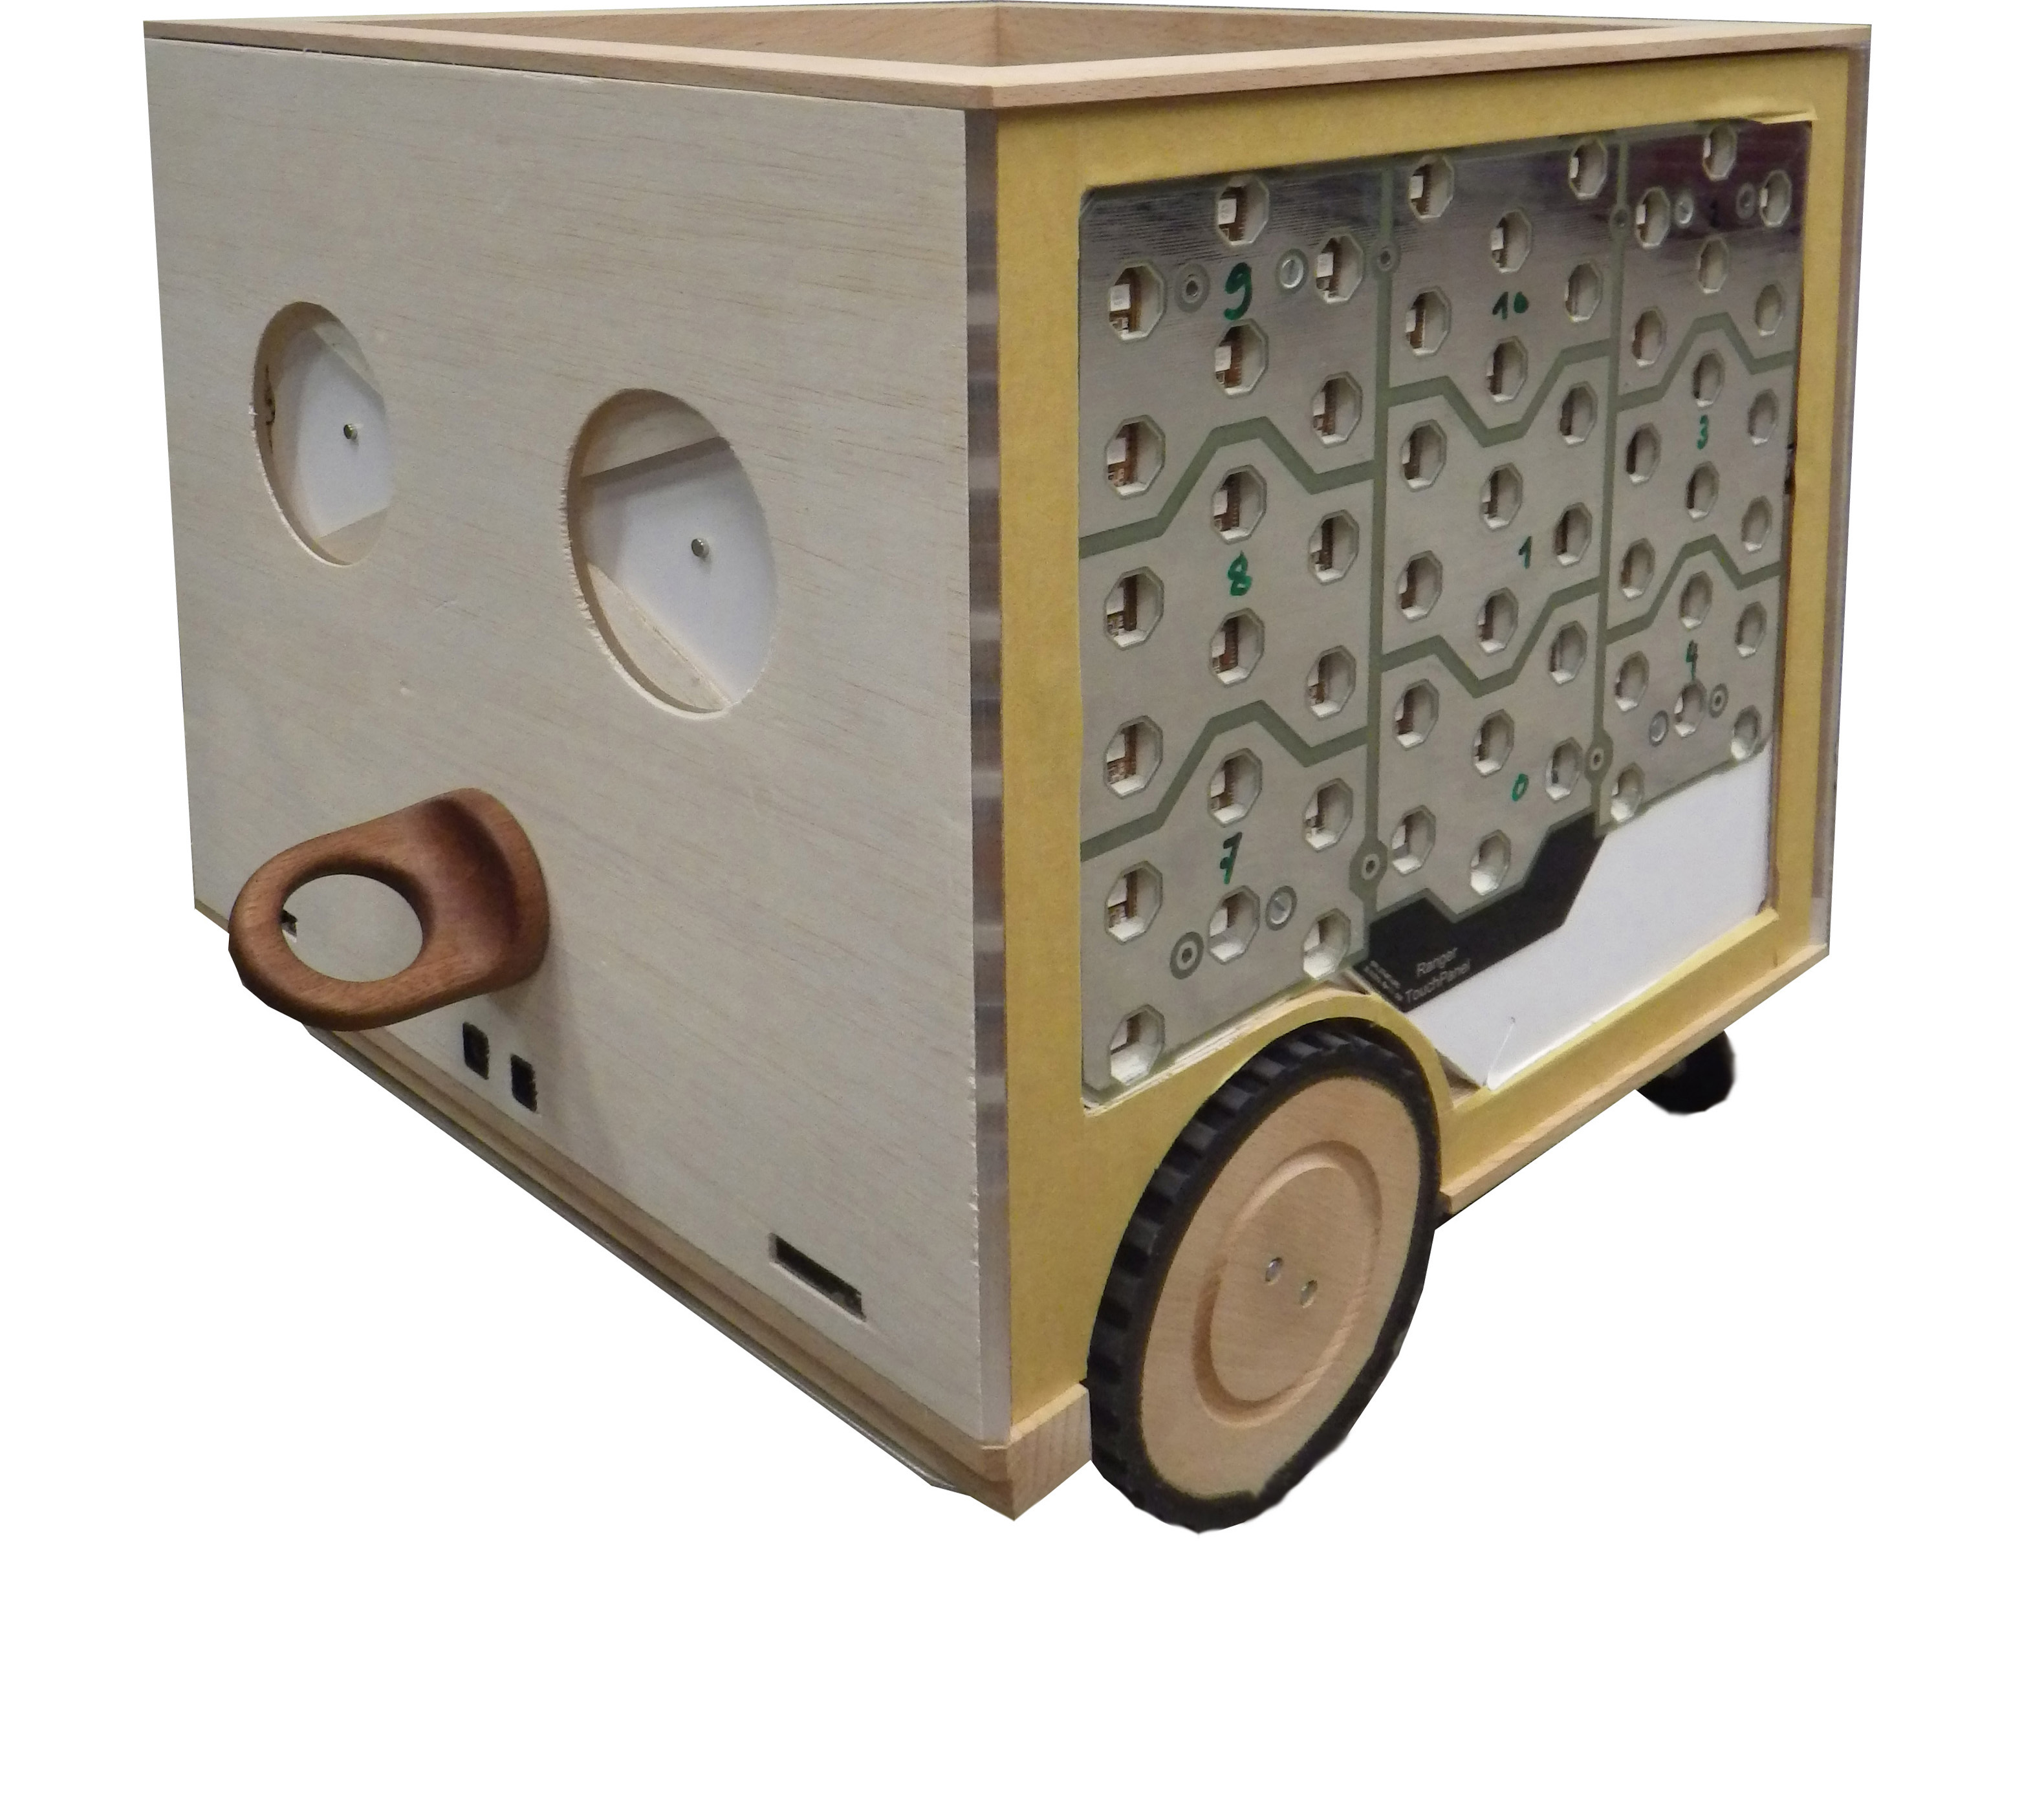
\includegraphics[width=0.4\textwidth]{ranger-v3}};
            \coordinate (ue) at (-2.5,-1.2);
            \coordinate (pup) at (-2.5,-1.6);
            \coordinate (le) at (-2.5,-2);
            \coordinate (pac) at (-2.7,-3.3);
            \coordinate (irl) at (-2.7,-3.4);
            \coordinate (irc) at (-2,-4);
            \coordinate (irr) at (-1,-4.5);
            \coordinate (bump) at (-0.5,-5);
            \coordinate (grd) at (0,-5.2);

            \coordinate (sto) at (0,-0.3);
            \coordinate (touch) at (1.6,-1.5);
            \coordinate (imu) at (3,-2);
            \coordinate (leds) at (2.2,-2.5);
            \coordinate (caswhe) at (2.5,-3.85);
            \coordinate (rab) at (2,-4.1);
            \coordinate (whe) at (1.3,-4.9);


            \coordinate (leftcaption) at (-3.5,0);
            \coordinate (rightcaption) at (3.5,0);

            \node[below=0.5 of leftcaption, anchor=east] (c-ue) {Upper eyelid} edge [->] (ue);
            \node[below=0.5 of c-ue.south east, anchor=east] (c-pup) {2-DoF pupil} edge [->] (pup);
            \node[below=0.5 of c-pup.south east, anchor=east] (c-le) {Lower eyelid} edge [->] (le);
            \node[below=0.6 of c-le.south east, anchor=east] (c-pac) {Removable pacifier} edge [->] (pac);
            \node[below=1.0 of c-pac.south east, anchor=east] (c-ir) {IR sensors} edge [->] (irl);
            \draw[->](c-ir) -- (irc);
            \draw[->](c-ir) -- (irr);
            \node[below=0.5 of c-ir.south east, anchor=east] (c-bump) {Bumper} edge [->] (bump);

            \node[above=0.2 of rightcaption.south west, anchor=west] (c-sto) {Toys storage and scale} edge [->,bend right] (sto);
            \node[below=1 of c-sto.south west, anchor=west] (c-touch) {Capacitive touch array} edge [->] (touch);
            \node[below=0.5 of c-touch.south west, anchor=west] (c-imu) {Inertial sensors and sound} edge [->] (imu);
            \node[below=0.5 of c-imu.south west, anchor=west] (c-leds) {RGB LED array} edge [->] (leds);
            \node[below=0.5 of c-leds.south west, anchor=west] (c-caswhe) {Castor wheels} edge [->] (caswhe);
            \node[below=0.5 of c-caswhe.south west, anchor=west] (c-rab) {Range \& Bearing sensor} edge [->] (rab);
            \node[below=0.5 of c-rab.south west, anchor=west] (c-whe) {Wheels} edge [->] (whe);


        %\draw[help lines] (-5,-5) grid (5,0);
    \end{tikzpicture}

    \caption{The ranger robot main components and their locations. The eyeglasses
    have been removed for the purpose of the illustration.}

    \label{fig:ranger_c} 
\end{figure*}

\section{The ranger robot}
\label{sec:ranger} 

The \textit{ranger} robot (see figure~\ref{fig:ranger_room}) is based on a
common object that can be found in every children room: a wooden storage box for
toys.  This object has been transformed into what we call a \textit{robject},
i.e. an object augmented with robotic features.  This transformation has beed
carried out by an interdisciplinary team including mechatronic engineers,
interaction designers, ethnographers and roboticists.  The goal of this
\textit{augmentation} or \textit{robotization} of the object is to improve the
functionalities (using competences in robotics and mechatronics) by building on
the top of an existing interaction and affordance (using competences in
interaction design) and create a new form of robot that can be accepted in an
existing ecosystem (using competences in ethnography).

The resulting \textit{ranger} robot has a body based on the original wooden box
but is equipped with wheels, mechanical eyes, inertial sensors, distance
sensors, ground sensors, a bumper, an inside balance, capacitive external touch
sensors, LED panels behind the wooden surface, sound, eyeglasses, a detachable
pacifier and a range-and-bearing (R\&B) system to detect other rangers, the
battery charger and a beacon to know where the play zone is (see
figure~\ref{fig:ranger_c} for most details and figure~\ref{fig:ranger_room} for
a global view).  Its body is shaped to support a very specific interaction aimed
at encouraging the children to tidy up their room.  Instead of maximizing the
robotics functionalities for this type of application, the optimization is made
at a higher level, taking into account the capabilities of the children, the
ecosystem and the possible interaction.  Therefore, we made the choice to not
equip the \textit{ranger} with arms, for instance, because this adds complexity
and cost that can be avoided using the right form of interaction.  The new
\textit{robject}  is supposed to remain helping and interacting with the
children instead of becoming a tool that does a task on its own.  Finally, by
keeping a role close to the original storage box, the \textit{ranger} increases
its acceptance by the children and their parents.

The internal architecture of the robot is illustrated in figure
\ref{fig:ranger_s}.  The \textit{ranger} has four processors.  The main one is a
full embedded computer running Linux and providing the main wireless
connectivity, data storage and sound management.  Three micro-controllers,
connected using a CAN bus, manage the real-time part of the robot, including
power, sensors and actuators.  The ASEBA framework \cite{ASEBA} is used to
control the whole system and makes the link with ROS controllers.  Slam and
navigation are implemented using ROS.

The shape of the ranger has been designed to keep a neutral wooden surface that
can become a projection surface from inside.  The 186 RGB LEDs that can project
light on this surface can create a large set of animated patterns.  The eyes are
fully mechanical, without any screen, creating a coherent image of real device.
The eyelids allow to give more expression and close the eyes when inactive.  The
eyeglasses of different colors allow a protection of the mechanics of the eyes
and at the same time allow a distinction among the several rangers holding
several types of toys, for instance.  The pacifier is also made of wood but
includes a magnet to be placed in the ``mouth'' of the rangers.  For some
experiments we add a RGDB Primesense sensor connected by USB to the Linux board
and helping in navigation and obstacle detection.

\begin{figure*}[ht]
 \centering
    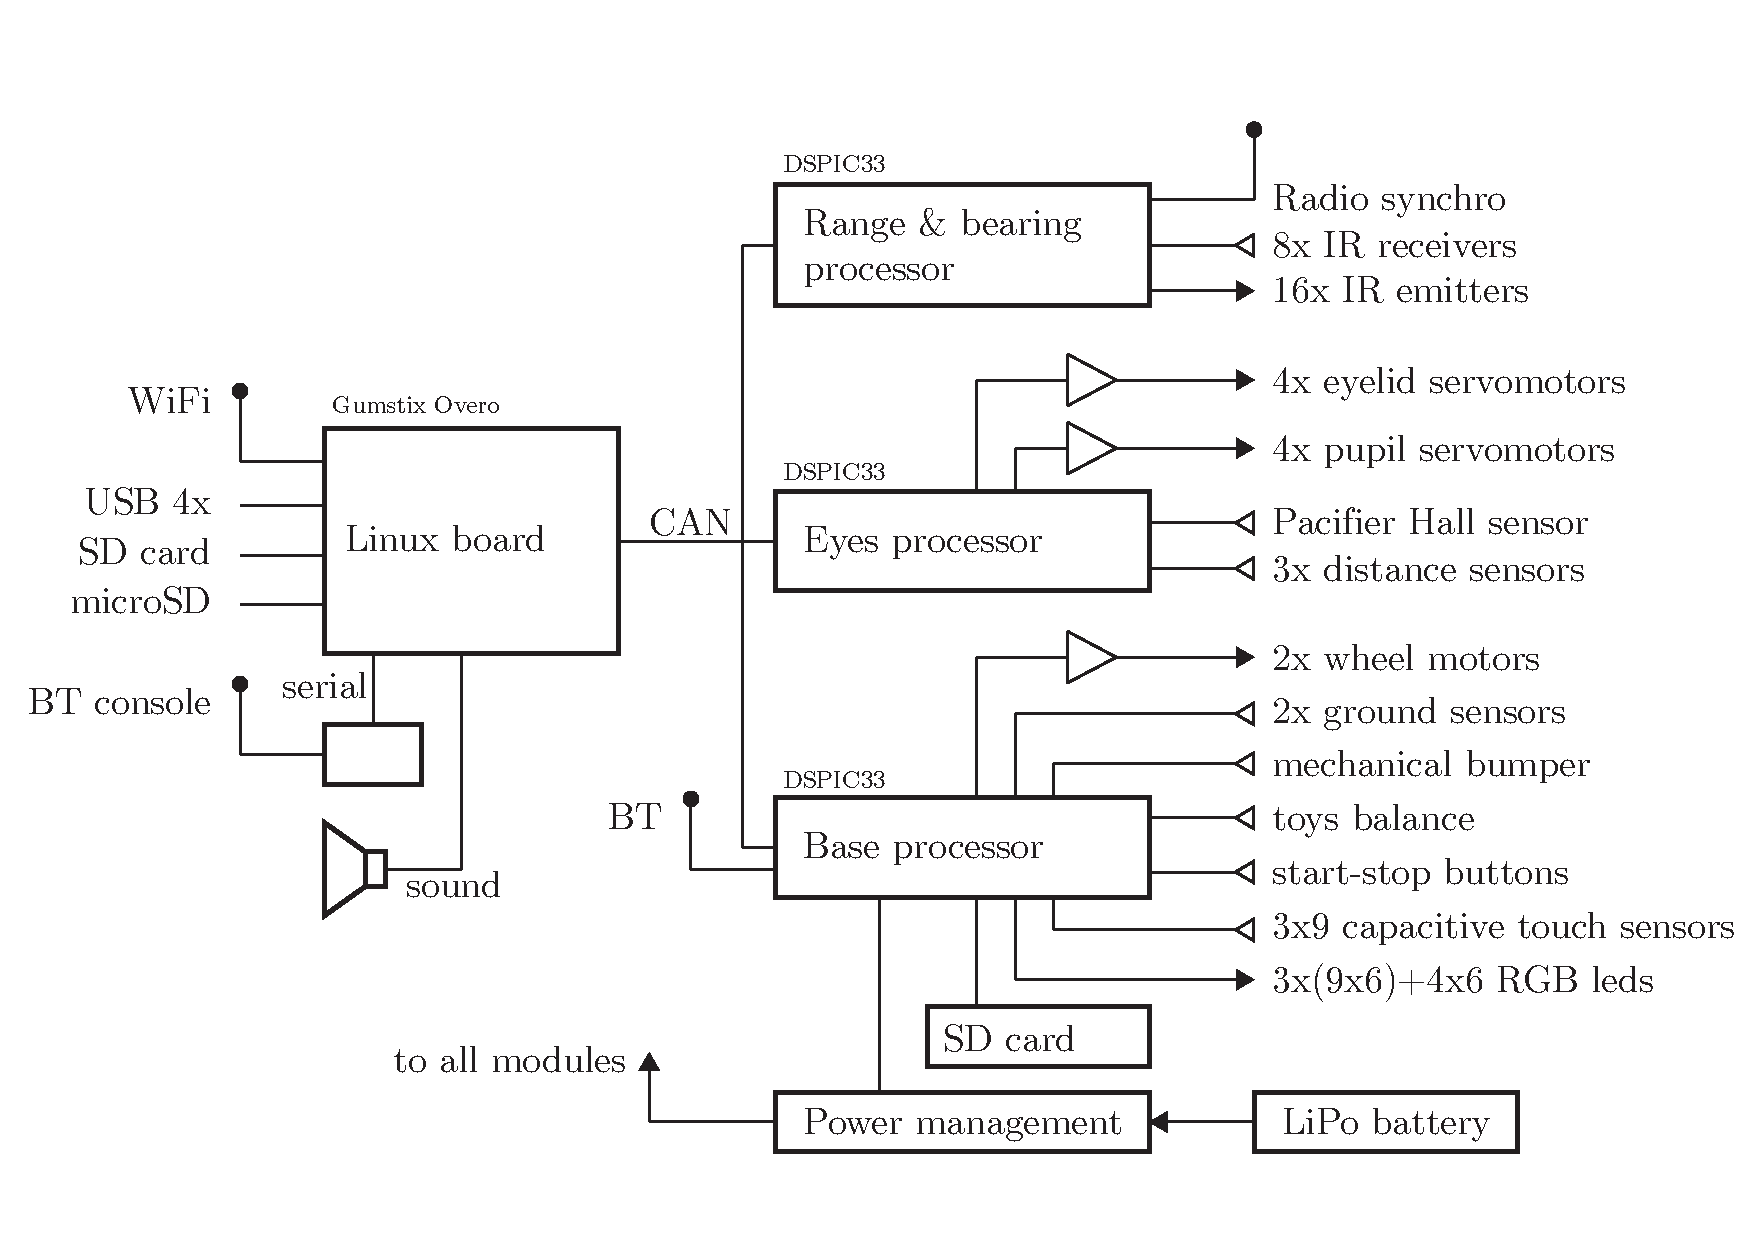
\includegraphics[width=0.9\columnwidth]{system-scheme.pdf}
  \caption{The structure of the electronics of the ranger robot. Four processors
  manage the functionalities and can be expanded using the USB ports of the
  Linux board.}
  \label{fig:ranger_s} 
\end{figure*}

\subsection{Ranger use scenario}
\label{sec:rangeruse} 

The use scenario is based on a room equipped with a bed under which several
rangers can be stored (see figure \ref{fig:ranger_room}).  Under the bed we
placed, for each ranger, a recharging station equipped with a R\&B beacon.  This
is the home of the rangers where they sleep, with closed eyes, most of the time.
Their behavior is defined by a state machine.  Figure \ref{fig:ranger_behav}
shows a simplified version of the state machine controlling the ranger behavior. 

\begin{figure*}[ht]
    \centering
    \begin{tikzpicture}[
        >=latex]
        \node[anchor=north east] at (-1,0){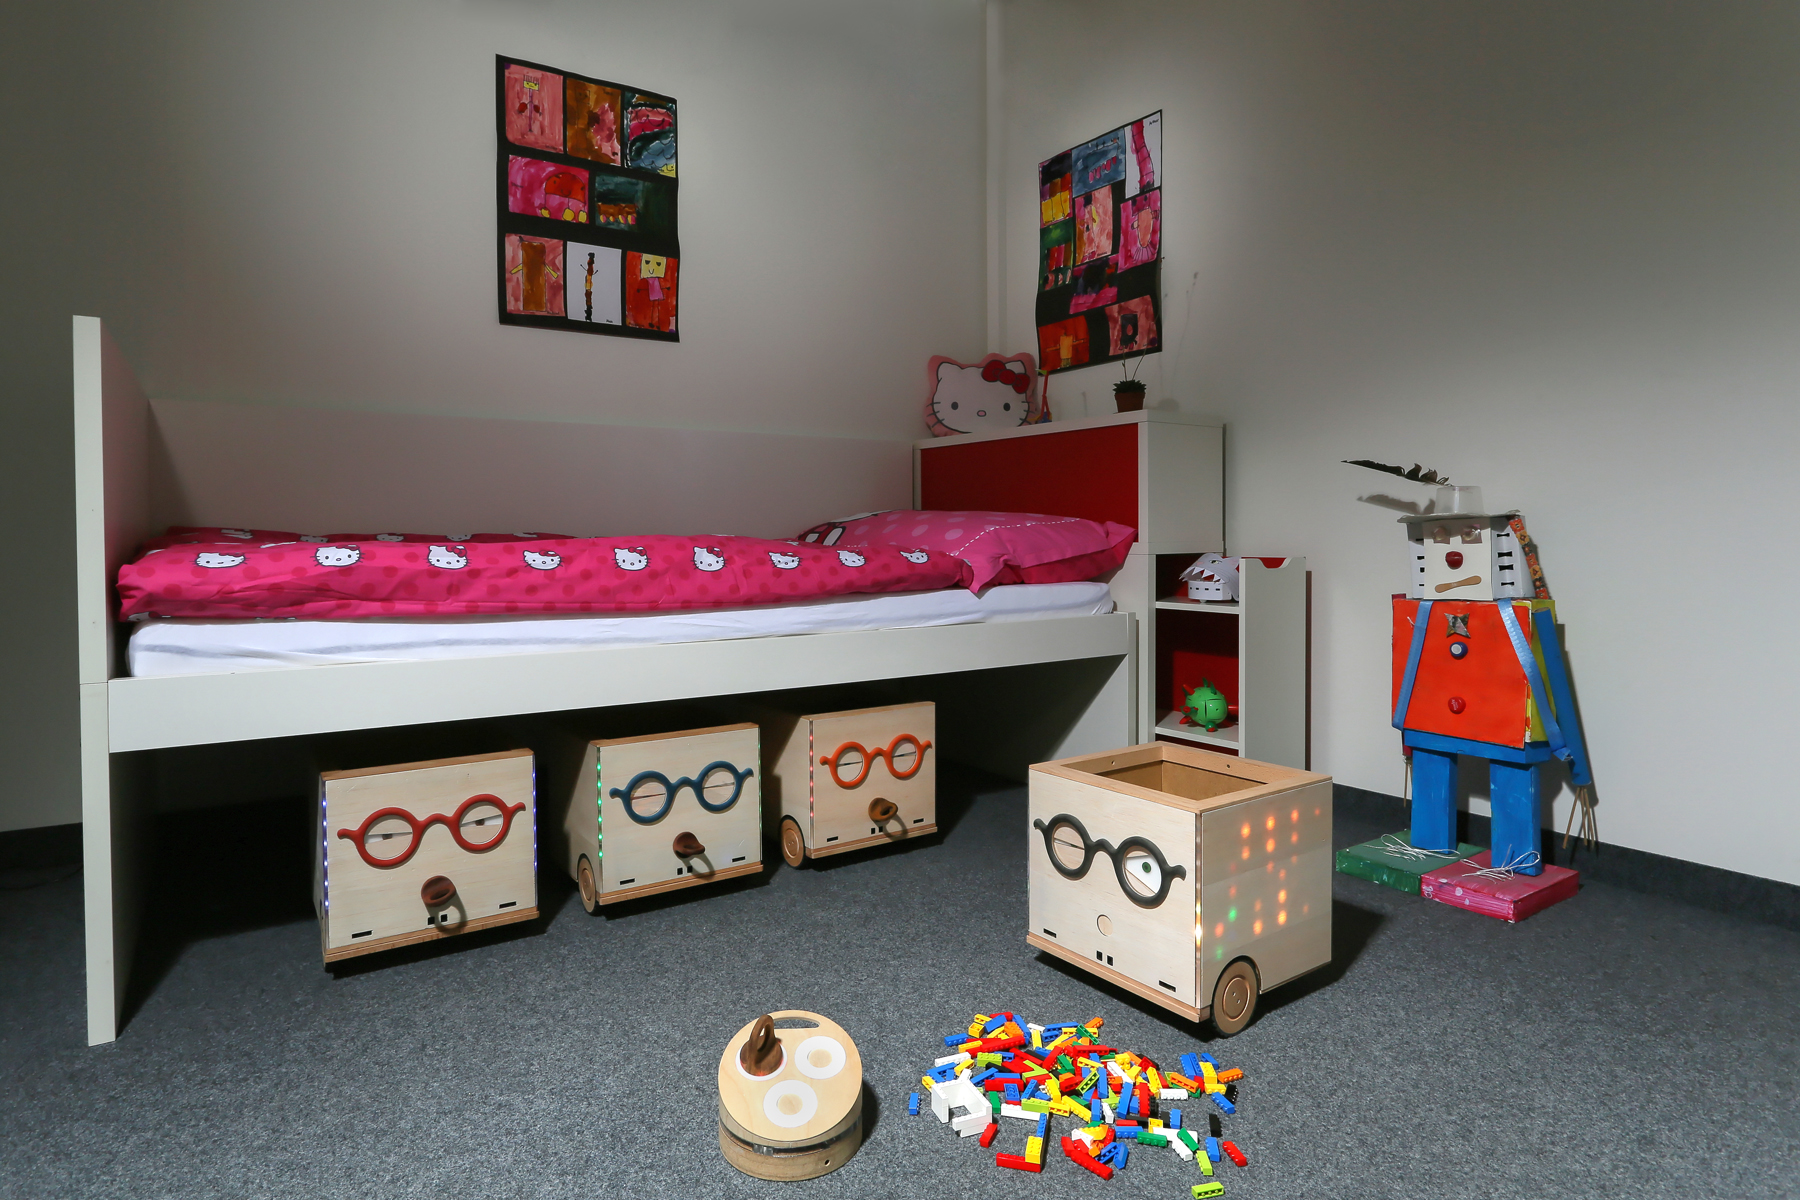
\includegraphics[width=0.3\textwidth]{ranger-room}};
        
        \node[circle, draw, thick] at (0,0) (1) {1};
        \node[circle, draw, thick] at (5,0) (2) {2} edge[<->] node[above] {(collective) navigation} (1);

        \node[rectangle, draw, below=1.4 of 1, align=center](a) {Sleeping\\home};
        \node[rectangle, draw, below=0.3 of 2](b) {Playing};
        \node[rectangle, draw, below=0.3 of b](c) {Waiting};
        \node[rectangle, draw, below=0.3 of c](d) {Starving};
        \node[rectangle, draw, below=0.3 of d](e) {Sent home};

        \path[->, bend left] (a) edge node[sloped, above] {pacifier removed} (b)
                             (b.east) edge (c.east)
                                      edge (e.east)
                             (c.west) edge (b.west)
                             (c.east) edge (d.east)
                                      edge (e.east)
                             (d) edge (a)
                             (e) edge node[sloped, below] {pacifier in slot} (a);


        %\draw[help lines] (-5,-5) grid (5,0);
    \end{tikzpicture}

  \caption{The behavior of the ranger is based on two positions: under the bed
  (home) and on the playing site. At home the ranger can be charged and the
  playing site is marked by a beacon where the children place the pacifiers.}
  \label{fig:ranger_behav} 
\end{figure*}

The children have a controller object (called ``collector'') where they can
place up to three pacifiers.  This collector of pacifiers can be seen on the
bottom, center, of figure \ref{fig:ranger_room}.  The collector is equipped with
a beacon.  To play with their toys, the children identify which ranger hold
them. Each ranger has a different color of glasses.  The child can wake up the
right ranger by taking away the pacifier from its mouth.  The child then puts
the pacifiers in the collector placed where the children want to play.  The
ranger will wake up and navigate toward the collector beacon.  Once the child
wants to send back the ranger home, he can simply put again the pacifiers in its
``mouth'' and the ranger will go back home to sleep (and recharge).  The ranger
can also decide to go back home if it sees that the battery level is too low.  A
set of behaviors is used to keep the child engaged.  It is motivated to tidy up
and fill ranger by the robot showing signs of hunger and sadness if he not being
"fed" - while displaying happiness as a rewarding behavior if toys are being
placed inside ranger.

\subsection{Validation}
\label{sec:validation} 

We tested the ranger concept in 14 families in a first short-term study
\cite{Fink2014}.  One ranger prototype was placed in the room of the children
while a researcher was discussing with the family in another room.  The family
was then asked to go in the room of the children and discover the ranger.  The
ranger was remotely controlled from a third room through a hidden camera,
following a predefined scenario describing the behavior, following a
Wizard-of-Oz methodology \cite{green1985rapid}.  In half of the families we
adopted a reactive behavior, with the ranger waiting for actions of the children
before reacting.  In the other half we adopted a proactive behavior, with the
ranger proactively moving and looking for objects on the ground.

\begin{figure*}[ht]
 \centering
    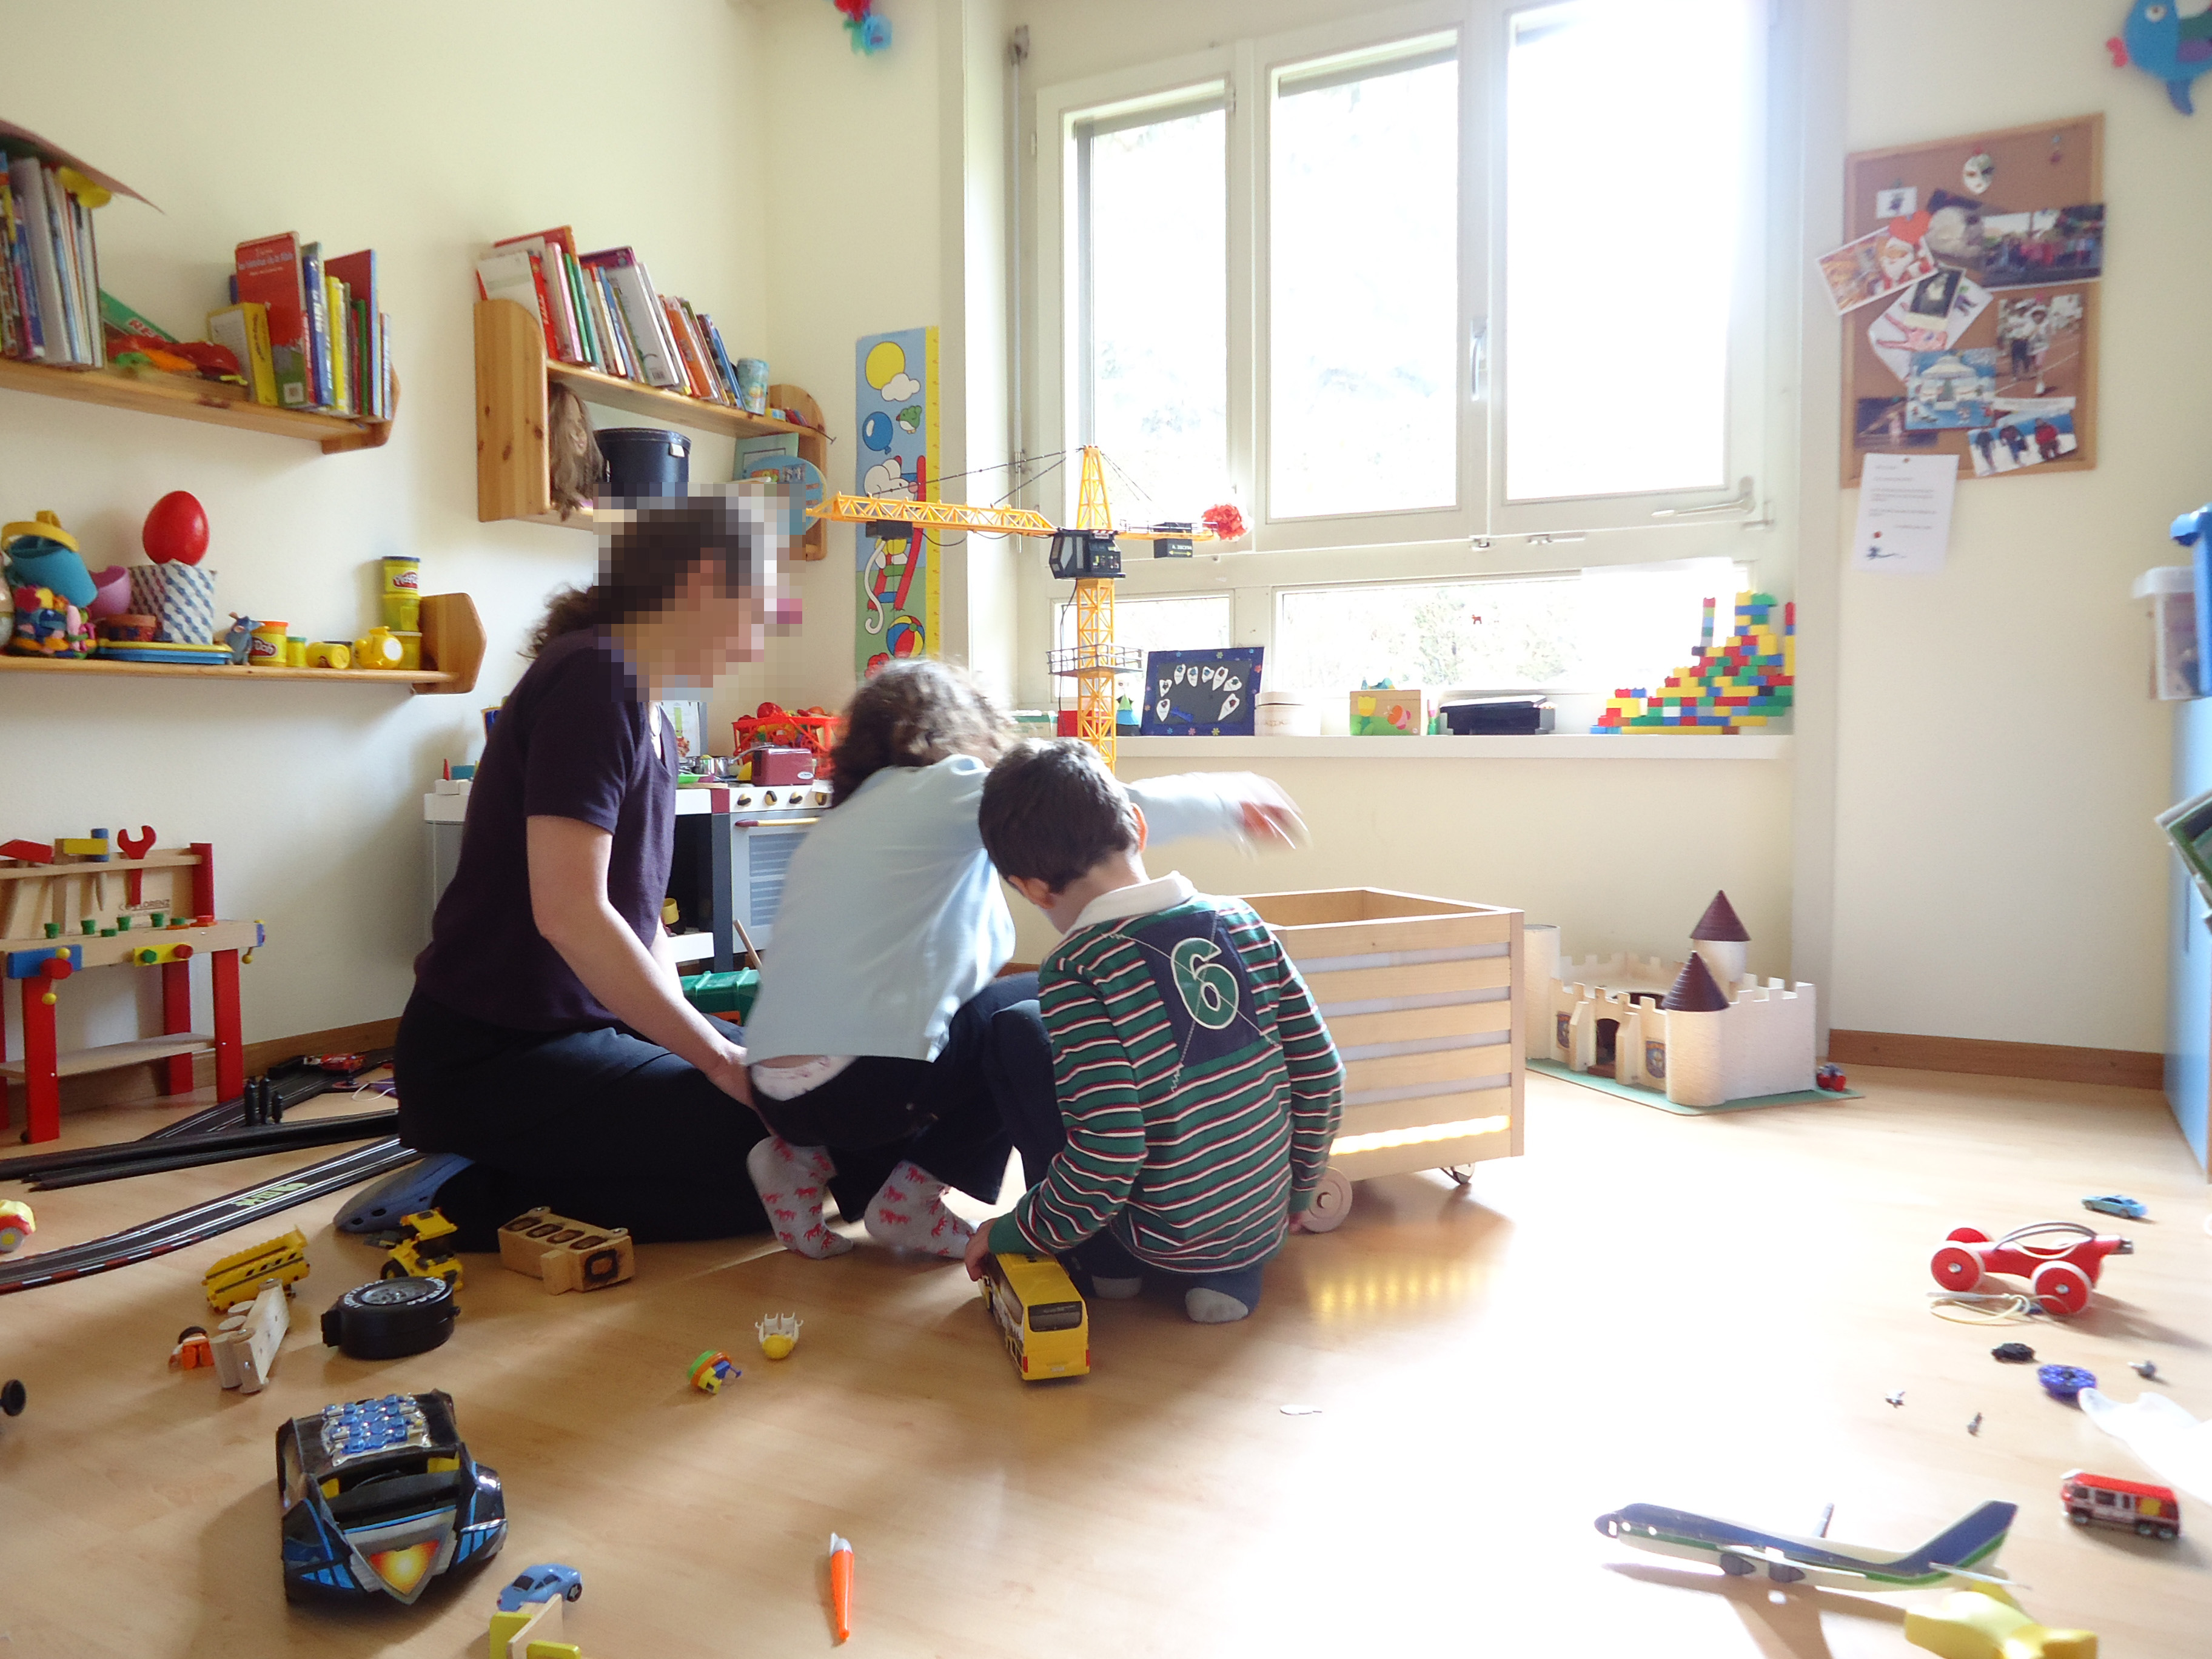
\includegraphics[height=6cm]{family-ranger.jpg}
  \caption{An image taken during user tests in families.}
  \label{fig:validation} 
\end{figure*}

These tests have shown a very high acceptance, as illustrated by the detailed
results presented in \cite{Fink2014}.  Moreover we observed that marginally
significantly more toys were put and removed in the reactive compared to the
proactive behavior.  This demonstrates that the robot can achieve good
performances even with a minimalist behavior. 

The next step consists in making tests with users in a configuration similar to
the one presented in figure \ref{fig:ranger_room} and for a long period, to see
to what extent users engage in using the ranger after novelty effects have worn
off.



\section{Conclusion}

We presented the concept and design of the ranger robot, a robotic storage box
that can interact with children to motivate them to tidy-up their room.  This
concept is very similar to the one adopted by several successful industrial
robotics systems that have shown the path of a smart integration of human and
robotic activities, limiting the requirements for the robotic technology and
improving performances thanks to a good human-robot cooperation.  Following this
design approach, we can design robots that fit with the factors identified by
Bauwens et al. \cite{Bauwens2012}: practical utility, integration in the
ecosystem and economic utility.  The validation in families has shown that
\textit{ranger} achieves high acceptance rates and a good utility in short-time
experiments.  In parallel, this test shows that good performances can be
achieved with a minimal behavior, helping to reach the economic utility.  These
results are achieved because of the embodiment into a daily-life object,
ensuring an optimal affordance and integration into the home ecosystem.  This
example illustrates the potential of the \textit{robjects} concept but also
shows that this concept requires an holistic approach that integrates
interaction design, robotics and mechatronics design. 

\section*{Acknowledgment}

This work was supported by the Swiss National Center of Competence in Research
"Robotics"


\bibliographystyle{abbrv}
\bibliography{ranger}


\end{document}
